\subsection{Cache Performance Analysis}
\label{sec:nehalem}

\begin{figure}[hbt!]
\centering
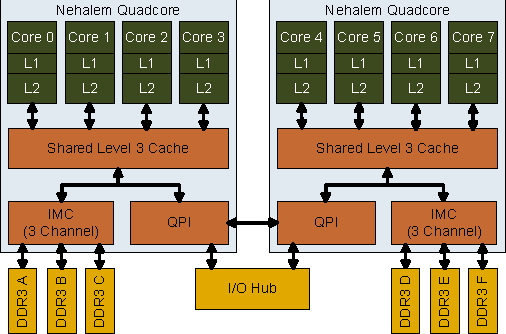
\includegraphics[width=0.6\columnwidth]{\chapterdirectory/figure/micro_bench/intel_nehalem.pdf}
\caption{%
Interconnected Intel Nehalem processors (extracted from \cite{10.1109/PACT.2009.22}).
}
\label{fig:micro_bench:intel_nehalem}
\end{figure}

\cite{10.1109/PACT.2009.22} is a paper on benchmarks performed on the Intel
Nehalem architecture (see Figure~\ref{fig:micro_bench:intel_nehalem}), which
uses the MESIF cache coherence protocol and has an inclusive cache hierarchy.
For clarification's sake, the cache coherence protocol is active below the L3
cache, meaning that this dual processor architecture effectively results in
only two caches being made coherent through MESIF.

To perform the benchmarks comparing the effect of coherence states of memory
element on writing and reading performance, their benchmark library makes it so
they are able to put data in the desired stable coherence state in the cache
they want, potentially using the other processor to attain the desired state.
In effect, this allows control of the coherence states of the system prior to
the start of the benchmark.  To reach the desired state in the caches of core
$N$, the following strategy is employed:
\begin{description}
\item[Modified] Core $N$ writes the data.
\item[Exclusive] Core $N$ writes the data (thus invalidating the other cores'
data), flushes, then reads the data.
\item[Shared] Core $N$ reaches the \textit{Exclusive} state, then another core
reads the same data.
\end{description}

There is an interesting omission: the \textit{Forward} state is not considered.
The authors indicate expecting the \textit{Forward} state to only become an
improvement for systems in which there are more than two processors and is thus
assumed not to have any effect on the benchmarks of their dual processor
architecture. This is incorrect, but, as explained later, the effects of the
\textit{Forward} are not seen in their results, since the benchmarks which would
have been affected were also omitted.

On the other hand, the strategy to reach a selected state for core $N$ described
above is still valid, even when ignoring the \textit{Forward}. Indeed, with this
process, the \textit{Forward} state only appears when reaching the
\textit{Shared} state, but it is reached by the core that ``reads the same
data'', not core $N$. In reality, having a \textit{Forward} state in an
architecture with only two caches does actually have some benefits: if the two
caches have read certain data, then one wants to write to it. Without
\textit{Forward} state, the cache wanting to write will have to fetch data in
RAM, whereas with the \textit{Forward} state available, it might be provided by
the other cache or simply ot have to fetch it in RAM (depending on which cache
performed a write first, and choices of implementation). Similarly, it has an
impact if a cache line is read by both caches, but the cache not in the
\textit{Forward} cache evicts it at some point, them re-acquires it. This would
have had an observable result when measuring the writing execution time. Indeed,
writing when core $N$ is in the \textit{Shared} state and another core is in the
\textit{Forward} state should result in faster execution time than when the other core
is in the \textit{Shared} state. Since The paper does not feature a table
proving a list of execution time when writing, but only for benchmarks that reading,
this difference cannot be seen and one might erroneously assume that the
\textit{Forward} state does indeed have no impact on systems with coherence
maintained between only two caches.

\iffalse
Considerations are taken to minimize any mechanic interfering with the
benchmarks: transaction look-aside buffers are pre-loaded and accessed memory
elements are not adjacent to avoid any pre-fetching optimization.
\fi

\begin{figure}[hbt!]
\begin{tabular}{cc}
\begin{subfigure}[t]{0.47\textwidth}
\lstinputlisting{\chapterdirectory/figure/micro_bench/algo_nehalem_latency.txt}
\caption{Latency benchmarks}
\label{fig:micro_bench:intel_nehalem_latency_algo}
\end{subfigure}
&
\begin{subfigure}[t]{0.47\textwidth}
\lstinputlisting{\chapterdirectory/figure/micro_bench/algo_nehalem_bandwidth.txt}
\caption{Bandwidth benchmarks}
\label{fig:micro_bench:intel_nehalem_bandwidth_algo}
\end{subfigure}
\end{tabular}
\caption{%
Algorithm overview for \cite{10.1109/PACT.2009.22} (taken from the paper)
}
\label{fig:micro_bench:intel_nehalem_algo}
\end{figure}

Figure~\ref{fig:micro_bench:intel_nehalem_latency_algo} shows an overview of the
algorithm used by \cite{10.1109/PACT.2009.22} to measure execution times. The steps
described are more about what is done prior to the measurements themselves.
Warming up the transaction look-aside buffer means pre-loading all entries in
order to avoid this loading being taken into account in the resulting execution time.
The accesses made for the measured part of the benchmark correspond to a pointer
chasing algorithm, just like in \cite{10.1145/2086696.2086713} (see
Figure~\ref{fig:micro_bench:co_running_apps_cots_algo_part_deux}).

The bandwidth benchmarking algorithm is shown in
Figure~\ref{fig:micro_bench:intel_nehalem_bandwidth_algo}. Synchronization
between the threads is more thoroughly controlled in this one: by memorizing the
exact window upon which each thread made its accesses, the window corresponding
to the period in which all threads were performing accesses can be obtained.
The bandwidth can then be obtained from the number of accesses successfully
performed within this window.

\begin{figure}[hbt!]
\centering
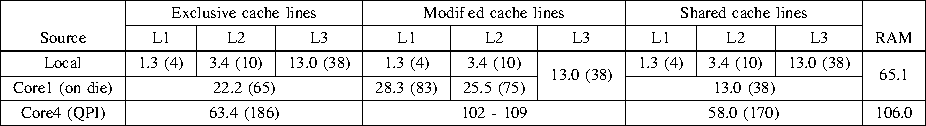
\includegraphics[width=\textwidth]{\chapterdirectory/figure/micro_bench/nehalem_read_latencies.pdf}
\caption{%
Latencies of reading from Core 0, results in ``nanoseconds (cycles)'' (Figure
taken from \cite{10.1109/PACT.2009.22})
}
\label{fig:micro_bench:intel_nehalem_read_latencies}
\end{figure}

Figure~\ref{fig:micro_bench:intel_nehalem_read_latencies} shows the results of
benchmarks measuring the time required for the core 0 to read data held in
various locations, according to the state of the data in the remote location.
Unsurprisingly, accesses made to the local L1 and L2 caches was not impacted by
the state of the data in the L3 cache. It appears this also holds true for the
local L3 cache itself. Access to data held in the caches of another core on the
same processor does vary depending on the coherence state. According to
\cite{10.1109/PACT.2009.22}, this is explained by the L3 cache having to check
on the L2 and L1 caches of that other core, as, unless the state is
\textit{Shared}, the L1 and L2 cores may hold a more up-to-date value. For data
held in the other processor, the results are as expected, with the cost of
traversing the bridge between both processors being added when accessing memory
elements in either the \textit{Exclusive} or \textit{Shared} state, but also
having a higher cost when accessing \textit{Modified} memory elements: as
explained in \cite{10.1109/PACT.2009.22} and Chapter~\ref{cha:cache_coherence},
\textit{Modified} memory elements are wrote back to the memory prior to being
sent as a reaction to a \textit{GetS} query.

\begin{figure}[hbt!]
\centering
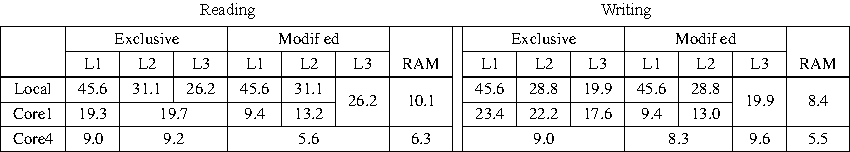
\includegraphics[width=\textwidth]{\chapterdirectory/figure/micro_bench/nehalem_bandwidths.pdf}
\caption{%
Bandwidth for access from Core 0, results in GB/s (Figure
taken from \cite{10.1109/PACT.2009.22})
}
\label{fig:micro_bench:intel_nehalem_broad}
\end{figure}

\cite{10.1109/PACT.2009.22} does however perform more analyses on the
performance of cache accesses. The second half of the paper is dedicated to
bandwidth analysis, of which the results are shown in
Figure~\ref{fig:micro_bench:intel_nehalem_broad}. These results are coherent
with their equivalent in the execution time benchmarks. They do provide more
information than what was available in the documentation however, such as actual
maximum bandwidth instead the theoretical maximal one.

The approach presented in \cite{10.1109/PACT.2009.22} is a good solution for the
\textit{benchmark} part of the framework described in
Section~\ref{sec:second_intro:framework}. Indeed, by taking into account the
coherence state of the targeted memory elements, \cite{10.1109/PACT.2009.22}
ensures the system state that led to the recording of the execution time is
understood and thus, that the correct execution time will be expected when attempting
to predict the architecture's behavior.
\stopallthesefloats
